\documentclass[times,english,brazil,oneside]{ifes7}

\usepackage[utf8]{inputenc}
\usepackage{lastpage}           % Usado pelo exemplo de ficha catalográfica
\usepackage[alf]{abntex2cite}
\usepackage{microtype}          % para melhorias de justificação
\usepackage{morefloats}         % permite mais floats
\usepackage{listings}
\usepackage{blindtext}          % para gerar texto aleatório (dummy text)
\usepackage{tikz}
\usetikzlibrary[topaths]
\usepackage{mathtools}
\usepackage{xcolor}


%%% Definição da linguagem padrão do documento (pacote babel) para
%%% definir que certas porções do texto (como o resumo, por exemplo)
%%% estão em uma língua estrangeira, usar as macros
%%% \foreignlanguage{languageB}{Text in another language}
%%% ou
%%% \begin{otherlanguage}{languageB}
%%% ...
%%% \end{otherlanguage}
\selectlanguage{brazil}


%%% Define que todos os códigos fontes construídos com o ambiente
%%% `lstlisting' terão uma borda simples.
\lstset{frame=single}


\newcommand{\ifestex}{\textsf{Ifes$7$}}

\titulo{Confecção de Monografias para Trabalhos de Conclusão de Curso
  no Ifes --- \emph{Uma Abordagem Utilizando Classes de Preparação de
    Documentos em \LaTeX2e}}

\autor{Alunus Alunovisk Alunovich}
\autorficha{Alunovich, Alunus Alunovisk}

\orientador{Prof. Dr. Jefferson O. Andrade}

\coorientador{Prof.ª Dr.ª Fulana Detal Longname}

\instituicao{Instituto Federal do Espírito Santo}

\curso{Bacharelado em Sistemas de Informação}

% \data{Fevereiro de 2016}
\data{2016}

\local{Serra}

\preambulo{Trabalho de Conclusão de Curso apresentado à Coordenadoria
  do Curso de Sistemas de Informação do Instituto Federal do Espírito
  Santo, Campus Serra, como requisito parcial para a obtenção do
  título de Bacharel em Sistemas de Informação.}

\tipotrabalho{Trabalho de Conclusão de Curso}



\begin{document}

%%% A macro \pretextual não precisa ser explicitamente chamada porque
%%% o abntex2 aciona essa macro no início do documento.
%%% \pretextual

\imprimircapa

\imprimirfolhaderosto*

\begin{fichacatalografica}
  \vspace*{\fill}
  % Posição vertical
  \begin{center}
    % Minipage Centralizado
    \fbox{
      \begin{minipage}[t]{12.5cm}
        \vspace*{3mm}
        \begin{minipage}[t]{2cm}
          X000x
        \end{minipage}
        \begin{minipage}[t]{10cm}
          \imprimirautorficha.\vspace{2mm}

          \hspace{0.5cm}\imprimirtitulo\ / \imprimirautor. ---
          \imprimirlocal, \imprimirdata.\\ 

          \hspace{0.5cm}\pageref{LastPage} p.:\ il. (algumas color.);
          30 cm.\\ 

          \hspace{0.5cm}\imprimirorientadorRotulo~\imprimirorientador.\\

          \hspace{0.5cm}\imprimirtipotrabalho\ ---
          \imprimirinstituicao, \imprimirdata\\

          \hspace{0.5cm}        
          1. Palavra-chave1.
          2. Palavra-chave2.
          I. Orientador.
          II. Universidade xxx.
          III. Faculdade de xxx.
          IV. Título.
          
          \begin{flushright}
            CDU 00:000:000.0
          \end{flushright}
          \vspace*{1mm}
        \end{minipage}
      \end{minipage}
    }
  \end{center}
\end{fichacatalografica}


%%% ====================================================================
%%% Exemplo de construção da folha de aprovação. Depois da
%%% apresentação do trabalho, quando a folha de apresentação real
%%% tiver sido assinada pela banca, a folha real deve ser digitalizada
%%% e o ambiente abaixo deve ser substituído por:
%%% \includepdf{folhadeaprovacao_final.pdf}
\begin{folhadeaprovacao}
  \begin{center}
    {\ABNTEXchapterfont\MakeTextUppercase{\imprimirautor}}\\
    \begin{center}
      \ABNTEXchapterfont\MakeTextUppercase{\imprimirtitulo}\\
    \end{center}
    \hspace{.45\textwidth}
    \begin{minipage}{.5\textwidth}
      {\footnotesize{\imprimirpreambulo}}\\
    \end{minipage}%
  \end{center}
  \vspace{-1cm}%
  \begin{center}
    Aprovado em 20 de fevereiro de 2016.\\[15mm]
    \textbf{COMISSÃO EXAMINADORA}\\[5mm]
    \assinatura{\imprimirorientador \\
      Instituto Federal do Espírito Santo \\
      Orientadora}\vspace{-1cm}
    \assinatura{\imprimircoorientador \\
      Instituto Federal do Espírito Santo \\
      Coorientador}\vspace{-1cm}
    \assinatura{Membro Convidado da Banca 1 \\
      Instituição Externa 1}\vspace{-1cm}
    \assinatura{Membro Convidado da Banca 2 \\
      Instituição Externa 2}
  \end{center}
\end{folhadeaprovacao}


%%% --------------------------------------------------------------------
%%% Ambiente para escrita da declaração do autor
\begin{declaracaodoautor}

  \vspace*{1.5cm}

  Declaro, para fins de pesquisa acadêmica, didática e
  técnico-científica, que este Trabalho de Conclusão de Curso pode ser
  parcialmente utilizado, desde que se faça referência à fonte e ao
  autor.

  \vspace*{2.5cm}

  \centering

  \imprimirlocal, 29 de setembro de 2016.

  \vspace*{2.5cm}

  \imprimirautor

  \vspace*{\fill}
  
\end{declaracaodoautor}


%%% ====================================================================
%%% Ambiente para a escrita da dedicatória.
\begin{dedicatoria}
  \vspace*{\fill}
  \hspace{0.2\textwidth}
  \begin{minipage}{0.8\textwidth}
    Este trabalho é dedicado aos que acreditam que Pikachu sempre será o
    melhor pokemon.
  \end{minipage}
\end{dedicatoria}


%%% ====================================================================
%%% Agradecimentos
\begin{agradecimentos}
  Agradeço a todos os que fizeram alguma coisa pela qual eu deveria
  ser grato.
\end{agradecimentos}


%%% ====================================================================
%%% Epígrafe
\begin{epigrafe}
  \vspace*{\fill}
  \begin{otherlanguage}{english}
    \begin{flushright}
      \begin{SingleSpace}
        People who think they know everything are a great \\
        annoyance to those of us who do. \cite{Asimov2004}
      \end{SingleSpace}
    \end{flushright}
  \end{otherlanguage}
\end{epigrafe}


%%% Ambiente para resumo em português
\begin{resumo}
  O objetivo deste documento é sevir como um modelo de trabalho de
  conclusão de curso tem por objetivo, bem como apresentar e descrever
  os mecanismos básicos para a confecção deste tipo de documento
  utilizando a classe de documentos \ifestex\ em \LaTeX.
  %
  Para uma melhor compreensão do modo de utilização desta classe é
  necessário analisar o código fonte deste documento bem como ler a
  documentação da classe \abnTeX, na qual a classe \ifestex\ se
  baseia.

  Palavras-chave: Palavra1. Palavra2. Palavra3. Palavra4.
\end{resumo}

%%% Ambiente para resumo em inglês.
\begin{resumo}[Abstract]
  \begin{otherlanguage}{english}
    The goal of this document is to work as a model for the
    undergraduate final year project report, as well as present and
    describe the basic mechanisms for the preparation of this type of
    document using the \LaTeX\ document class \ifestex.
    %
    To better understand how to use that class, it is necessary to
    study the source code of this document as well as read the
    documentation of the \abnTeX\ class, upon which the \ifestex\
    class is based.

    Keywords: Keyword1. Keyword2. Keyword3. Keyword4.
  \end{otherlanguage}
\end{resumo}


%%% Lista de figuras
\renewcommand{\listfigurename}{Lista de figuras}
\pdfbookmark[0]{\listfigurename}{lof}
\listoffigures*
\cleardoublepage


%%% Lista de tabelas
\pdfbookmark[0]{\listtablename}{lot}
\listoftables*
\cleardoublepage


%%% Lista de quadros
\pdfbookmark[0]{\listadequadrosname}{loq}
\listadequadros*
\cleardoublepage


%%% Lista de abreviaturas
\begin{abreviaturas}
\item[abrev.] abreviatura
\item[assoc.] associação
\item[atm.] atmosfera
\item[bel.] bacharel
\item[bioq.] bioquímica
\item[cit.] citação
\item[compl.] complemento
\item[dic.] dicionário
\item[dipl.] diploma
\end{abreviaturas}


%%% Lista de siglas
\begin{siglas}
\item[ABNT] Associação Brasileira de Normas Técnicas
\item[ACM] Association for Computing Machinery
\item[APA] American Psychological Association
\item[BIOS] Basic Input / Output System
\item[CREA] Conselho Regional de Engenharia e Agronomia
\item[IBGE] Instituto Brasileiro de Geografia e Estatística
\item[IEEE] Institute of Electrical and Electronics Engineers
\item[Ifes] Instituo Federal de Educação, Ciência e Tecnologia do
  Espírito Santo
\item[ISDN] Integrated Services Digital Network
\item[RISC] Reduced Instruction Set Computer
\end{siglas}


%%% Lista de símbolos
\begin{simbolos}
\simb{$\Gamma$} Letra grega Gama
\simb{$\Lambda$} Lambda
\simb{$\zeta$} Letra grega minúscula zeta
\simb{$\in$} Pertence
\simb{$\top$} Valor lógico máximo dentro de um reticulado regular
  booleano ou quasi-booleano.
\end{simbolos}
\cleardoublepage


%%% Sumário --- Table of Contents
\pdfbookmark[0]{\contentsname}{toc}
\tableofcontents*
\cleardoublepage


%%% ====================================================================
%%% Início da parte textual do documento.
\textual


%%% Configuração do espaçamento entre títulos e texto
\setlength{\afterchapskip}{1.5cm minus \baselineskip}


\chapter{Introdução}
\label{cha:introducao}

O Instituto Federal do Espírito Santo (Ifes) normatiza definições de
apresentação para trabalhos acadêmicos. À época da edição deste
documento (fevereiro de 2016), a norma mais recente é a 7ª edição,
publicada em 2014 \cite{Ifes2014}.

Com o objetivo de facilitar tanto o trabalho dos alunos na preparação
de seus Trabalhos de Conclusão de Curso (TCC), quanto o trabalho do
setor de bibliotecas, responsável pela validação da formatação dos
trabalhos entregues, foi solicitado que o Ifes disponibilizasse uma
classe e/ou modelo em \LaTeX\ que seguisse as normas de
apresentação. Com esse objetivo foi iniciado o trabalho de construção
da classe \ifestex.\footnote{A título de esclarecimento, caso não seja
  evidente, o autor deste documento é o Prof.\ Jefferson O.\ Andrade,
  o estudante \emph{Alunus Alunovisk Alunovich} é fictício.}

Este documento funciona ao mesmo tempo como manual e como modelo de
TCC para a classe \ifestex. Esta classe é essencialmente uma
customização da classe \abnTeX\ \cite{abntex2classe} -- que, por sua
vez, é uma extensão da classe \texttt{memoir}. Deste modo, este
manual/modelo, vai buscar, na medida do possível, não repetir o que já
está disponível no manual do \abnTeX\ ou nas normas do Ifes
\cite{Ifes2014}, e se concentrar no que é novo e/ou diferente na
classe \ifestex.

É altamente recomendável que os estudantes verifiquem, além da versão
em PDF deste documento, também o seu código fonte em \LaTeX.

\section{Uso Básico da Classe \ifestex}
\label{sec:uso-basico}

Para utilizar a classe \ifestex\ no seu trabalho acadêmico,
evidentemente, você precisará informar ao \LaTeX\ que está usando a
classe. Isso é feito colocando-se a declaração abaixo como a primeira
linha de código do seu documento.\vspace{\baselineskip}

\begin{lstlisting}[language={[LaTeX]TeX}]
  \documentclass[times,english,brazil]{ifes7}  
\end{lstlisting}

A opção \texttt{12pt} indica o tamanho padrão da fonte do texto,
conforme estabelecido pelas normas do Ifes \cite[pp.~20]{Ifes2014}.

A opção \texttt{a4paper} estabelece o uso de papel tamanho A4,
conforme definido em \cite[pp.~19]{Ifes2014}.

A opção \texttt{times} não é explicitamente necessária uma vez que ela
é o padrão. Essa opção faz com que a fonte padrão do documento seja
“Latin Modern” que é semelhante à “Times New Roman”, porém superior
tipograficamente. A opção complementar à \texttt{times} é a
\texttt{arial}. A opção \texttt{arial} faz com que a fonte padrão do
documento (inclusive para fórmulas matemáticas) seja a “Helvetica” que
é semelhante à “Arial”, porém superior tipograficamente.

As opções \texttt{english} e \texttt{brazil} são passadas ao pacote
\texttt{babel}, que é carregado automaticamente pela classe \abnTeX.
A classe \texttt{babel} redefine vários elementos do \LaTeX para
controlar questões relacionadas ao idioma do documento, tais como
nomes de alguns elementos textuais pré-definidos (``Figura'',
``Tabela'', etc.) e hifenização. A razão de incluir a opção
\texttt{english} é devido à necessidade de haver o resumo em língua
estrangeira. Caso o resumo esteja em outra língua estrangeira deve-se
usar a opção correspondente, como \texttt{french}, \texttt{spanish},
etc. É importante notar que, quando mais de uma opção de linguagem é
informada ao \texttt{babel} é preciso dizer ao babel no corpo do
documento que língua usar. Isso é feito colocando-se a seguinte linha
de código no documento:\vspace{\baselineskip}

\begin{lstlisting}[language={[LaTeX]TeX}]
  \selectlanguage{brazil}  
\end{lstlisting}

Além destas opções, qualquer opção válida para a classe \abnTeX\ pode
ser passada na declaração \texttt{documentclass}. As opções
específicas da classes \abnTeX\ serão passadas diretamente à ela.


\section{Uma Seção para Testar Listas Não Ordenadas}

\blindtext[1]

\begin{itemize}
\item Primiero item.
\item Segundo item.
  \begin{itemize}
  \item Primeiro sub-item.
  \item Segundo sub-item.
    \begin{itemize}
    \item Primeiro sub-sub-item.
    \item Segundo sub-sub-item.
    \item Terceiro sub-sub-item.
      \begin{itemize}
      \item Primeiro item do subnível 4.
      \item Segundo item do subnível 4.
      \end{itemize}
    \item Quarto sub-sub-item.
    \end{itemize}
  \item Terceiro sub-item.
  \end{itemize}
\item Terceiro item.
\item Quarto item.
\end{itemize}

\blindtext[2]


\section{Uma Seção sem Propósito}
\label{sec:sem-proposito1}

\Blindtext

\blinditemize[7]

\blindtext[2]

\blindenumerate[5]

\blindtext



% ----------------------------------------------------------------------
\chapter{Seção Primária}
\label{cha:secao-primaria}

\blindtext[1]

\section{Seção Secundária}
\label{sec:secao-secundaria}

\blindtext[1]

\subsection{Seção Terciária}
\label{sec:secao-terciaria}

\blindtext[1]

\subsubsection{Seção Quaternária}
\label{sec:secao-quaternaria}

\blindtext[1]

\paragraph{Seção Quinária}
\label{sec:secao-quinaria}

\blindtext[1]


% ---------------------------------------------------------------------
\chapter{Este é um Capítulo com Título Realmente Bastante
  Longo para Verificar o Alinhamento}


\blindtext



% ----------------------------------------------------------------------
\chapter{Formatação de Elementos Pré-textuais}
\label{cha:format-pre-text}

O manual do \abnTeX\ descreve bem a construção dos elementos
pré-textuais típicos de um trabalho acadêmico, disponibilizando macros
para a maioria deles, conforme pode ser verificado em
\cite[cap.~6]{Araujo2016}. Esses elementos, segundo as normas do Ifes
são:

\begin{enumerate}
\item Folha de rosto (obrigatório)
\item Ficha catalográfica (obrigatório)
\item Errata (opcional)
\item Folha de aprovação (obrigatório)
\item Declaração do autor (obrigatório)
\item Dedicatória (opcional)
\item Agradecimentos (opcional)
\item Epígrafe (opcional)
\item Resumo na língua vernácula (obrigatório)
\item Resumo em língua estrangeira (obrigatório)
\item Lista de ilustrações (opcional)
\item Lista de tabelas (opcional)
\item Lista de abreviaturas e siglas (opcional)
\item Lista de símbolos (opcional)
\item Sumário (obrigatório)
\end{enumerate}

Todos estes elementos tem suporte na classe \abnTeX, e a documentação
da classe deve ser consultada para mais informações sobre como usar
esse suporte \cite{Araujo2016}.

Este documento apresenta todas estas seções, construídas usando o
suporte da classe \abnTeX, e pode-se consultar o seu código fonte para
uma introdução rápida a este suporte.

A classe \ifestex\ redefine os comandos \verb!\imprimircapa! e
\verb!\folhaderostocontent! para adequar a capa e a folha de rosto aos
modelos indicados nos apêndices C e E, respectivamente, das normas do
Ifes \cite{Ifes2014}.



\chapter{Formatação de Elementos Textuais}
\label{cha:format-text}

A quantidade e o número de capítulos da parte textual ficam a cargo da
decisão do aluno e de seu orientador. Tipicamente a parte textual tem
entre 5 e 7 capítulos. Uma estrutura típica dos capítulos da parte
textual seria a seguinte:

\begin{SingleSpace}
  \begin{enumerate}
  \item Introdução
  \item Revisão Bibliográfica
  \item Especificação e Projeto
  \item Implementação
  \item Experimentos e Resultados
  \item Conclusões e Trabalhos Futuros
  \end{enumerate}
\end{SingleSpace}

Evidentemente, os títulos dos capítulos podem mudar e pode haver a
fusão de alguns capítulos, ou pode haver a divisão de alguns dos
capítulos em dois ou mais. Entretanto, não é comum haver um número
muito grande de capítulos.

A formatação dos títulos das seções do trabalho seguem as diretrizes
indicadas 4.3.7.1 das normas do Ifes \cite[p.~34]{Ifes2014}.
% , e a
% formatação dos títulos segue o seguinte esquema:

% \begin{description}
% \item[Capítulo] Maiúsculas, em negrito, tamanho \verb!\LARGE!.
% \item[Seção] Maiúsculas, tamanho \verb!\Large!.
% \item[Subseção] \emph{Smallcaps}, tamanho \verb!\large!.
% \item[Subsubseção] 
% \end{description}


\section{Formatação de Tabelas}
\label{sec:format-tabelas}

As normas do Ifes remetem ao documento ``normas de apresentação
tabular'' do Instituto Brasileiro de Geografia e Estatística(IBGE),
disponível em
\url{http://biblioteca.ibge.gov.br/visualizacao/livros/liv23907.pdf}.
Que é a mesma referência utilizada pelo \abnTeX. Assim, para atender
às normas do Ifes, basta utilizar a macro \verb!\IBGEtab!, conforme
explicado em \cite[p.~41]{Araujo2016}.

\begin{table}[h!]
  \IBGEtab{%
    \caption[Um Exemplo de tabela alinhada conforme padrão IBGE]{Um
      Exemplo de tabela alinhada que pode ser longa ou curta, conforme
      padrão IBGE.}%
    \label{tabela-ibge}
  }{%
    \begin{tabular}{ccc}
      \toprule
      Nome           & Nascimento & Documento      \\
      \midrule
      \midrule
      Maria da Silva & 11/11/1111 & 111.111.111-11 \\
      Júlia da Silva & 12/11/1111 & 111.111.112-22 \\
      Paulo da Silva & 13/11/1111 & 111.111.113-33 \\
      Pedro da Silva & 14/11/1111 & 111.111.114-44 \\
      \bottomrule
    \end{tabular}%
  }{%
    \fonte{Produzido pelos autores}%
    \nota{Esta é uma nota, que diz que os dados são baseados na
      regressão linear.}%
    \nota[Anotações]{Uma anotação adicional, seguida de várias outras.}%
  }
\end{table}

A Tabela~\ref{tabela-ibge}, é o mesmo exemplo apresentado no manual da
classe \abnTeX, inserida aqui apenas a título de demonstração.


\begin{quadro}[htb]
  \IBGEtab{
    \caption{Exemplo de uso de \texttt{cline} para formatação de
      tabelas.}
    \label{tab:ex2}
  }{
    \begin{tabular}{|r|l|}
      \hline
      7C0         & hexadecimal \\
      3700        & octal       \\ \cline{2-2}
      11111000000 & binary      \\
      \hline
      \hline
      1984        & decimal     \\
      \hline
    \end{tabular}
  }{
    \fonte{\LaTeX/Tables, Basic examples \cite{Wikibook-LaTeX}.}
  }
\end{quadro}

A Tabela~\ref{tab:ex2} ilustra o resultado o uso do comando
\verb!\cline! para criar linhas de separação (bordas) em apenas
algumas das colunas de uma tabela. Note que este exemplo consta apenas
para ilustrar as capacidades de formatação de tabelas do \LaTeX. As
normas do Ifes definem que \textbf{não deve haver} linhas horizontais
separando as linhas de dados, nem linhas horizontais separando as
colunas.

\begin{table}[h]
  \ibgetab{
    \caption[Exemplo de tabela em que é necessário quebras de
    linha.]{Exemplo de tabela em que o texto é muito grande para caber
      em uma única linha, e é necessário introduzir quebras de linha
      dentro da célula.}
    \label{tab:ex3}
  }{
    \begin{tabular}{lllp{5cm}}
      \toprule
      Day       & Min Temp & Max Temp & Summary                                                      \\
      \midrule
      Monday    & 11ºC     & 22ºC     & A clear day with lots of sunshine.  
                                        However, the strong breeze will bring down the temperatures. \\
      Tuesday   & 9ºC      & 19ºC     & Cloudy with rain, across many northern regions. Clear spells 
                                        across most of Scotland and Northern Ireland, 
                                        but rain reaching the far northwest.                         \\
      Wednesday & 10ºC     & 21ºC     & Rain will still linger for the morning. 
                                        Conditions will improve by early afternoon and continue 
                                        throughout the evening.                                      \\
      \bottomrule
    \end{tabular}
  }{
    \fonte{\LaTeX/Tables, Text wrapping in tables \cite{Wikibook-LaTeX}.}
  }
\end{table}

A Tabela~\ref{tab:ex3} apresenta um exemplo de tabela onde o texto em
uma das colunas é muito grande para caber nas células. Portanto é
necessário introduzir quebras de linha dentro das células. Uma forma
de se conseguir este efeito é indicar, como opção de formatação do
ambiente \texttt{tabular} o valor \verb!p{x}!, onde $x$ deve ser
substituído pela largura desejada para a coluna, por exemplo,
\texttt{5cm}. Outras opções podem ser obtidas com o uso dos pacotes
\texttt{tabularx} e \texttt{tabulary}.



\section{Formatação de Figuras}
\label{sec:format-figuras}

Não existe nada de excepcional sobre a formatação de figuras nas
normas do Ifes. Os únicos pontos que se deve prestar atenção é que o
título (\texttt{caption}) da figura deve ser colocado acima da figura
propriamente dita, e a fonte e notas/legendas devem vir abaixo da
figura.

\begin{figure}[h]
  \centering
  \caption{Diagrama de Venn indicando porque \LaTeX{} é melhor que M\$
    Word.}
  \label{fig:ex1}
  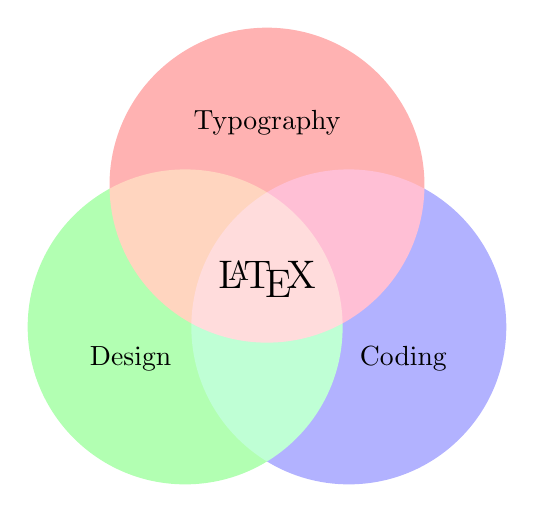
\begin{tikzpicture}
    \begin{scope}[blend group = soft light]
      \fill[red!30!white]   ( 90:1.2) circle (2);
      \fill[green!30!white] (210:1.2) circle (2);
      \fill[blue!30!white]  (330:1.2) circle (2);
    \end{scope}
    \node at ( 90:2)    {Typography};
    \node at ( 210:2)   {Design};
    \node at ( 330:2)   {Coding};
    \node [font=\Large] {\LaTeX};
  \end{tikzpicture}
  \fonte{A Venn Diagram for PDF blending \cite{Kottwitz2015}.}
  \nota{Este diagrama foi inteiramente feito com comandos \LaTeX,
    utilizando o pacote \texttt{tikz}, sem necessidade de qualquer
    outro software externo.}
\end{figure}

A Figura~\ref{fig:ex1} apresenta um diagrama de Venn que coloca o
\LaTeX como a interseção de três importantes áreas de conhecimento: a
tipografia, o \emph{design}, e a codificação. Essa representação faz
sentido pois o \LaTeX é ao mesmo tempo um ambiente de programação com
os algoritmos de tipografia mais sofisticados disponíveis ao usuário
doméstico e, caso se deseje, oferece extremo controle sobre todo o
\emph{design} do documento.

\begin{figure}[h]
  \centering
  \caption{Grafo completo com 16 nós.}
  \label{fig:ex2}
  \newcount\mycount
  \begin{tikzpicture}[transform shape]
    % the multiplication with floats is not possible. Thus I split the
    % loop in two.
    \foreach \number in {1,...,8}{
      % Computer angle:
      \mycount=\number
      \advance\mycount by -1
      \multiply\mycount by 45
      \advance\mycount by 0
      \node[draw,circle,inner sep=0.25cm] (N-\number) at
      (\the\mycount:5.4cm) {}; 
    }
    \foreach \number in {9,...,16}{
      % Computer angle:
      \mycount=\number
      \advance\mycount by -1
      \multiply\mycount by 45
      \advance\mycount by 22.5
      \node[draw,circle,inner sep=0.25cm] (N-\number) at
      (\the\mycount:5.4cm) {}; 
    }
    \foreach \number in {1,...,15}{
      \mycount=\number
      \advance\mycount by 1
      \foreach \numbera in {\the\mycount,...,16}{
        \path (N-\number) edge[->,bend right=3] (N-\numbera)
        edge[<-,bend left=3] (N-\numbera); 
      }
    }
  \end{tikzpicture}
  \fonte{A complete graph \cite{Quintin2012}.}
  \nota{Novamente, o diagrama foi completamente gerado em \LaTeX, sem
    a necessidade de recorrer a softwares externos. Note-se que o
    grafo possui $\frac{16\cdot(16-1)}{2}= 120$ arestas, esse número de arestas
    foi gerado programaticamente e não manualmente.}
\end{figure}

A Figura~\ref{fig:ex2} demonstra a capacidade de codificação que se
ganha ``de graça'' ao utilizar o \LaTeX. Consultando o código fonte
deste documento (ou a fonte da figura), pode-se notar que os nós e
arestas do grafo são gerados programaticamente e não manualmente como
seria necessário com o uso do M\$ Word ou do LibreOffice.


\section{Formatação de Equações e Fórmulas}
\label{sec:format-equac}

As normas do Ifes não estabelecem qualquer restrição maior quanto à
formatação de equações e fórmulas, exceto pelo fato de que devem ser
destacadas do texto e que, quando numeradas, a numeração deve ser
sequencial, com algarismos arábicos, entre parênteses e anumeração
deve ser alinhada à direita. Todos esses requisitos são
automaticamente obtidos quando se utiliza o ambiente \texttt{equation}
do \LaTeX.

\begin{equation}
  \label{eq:1}
  \cos (2\theta) = \cos^2 \theta - \sin^2 \theta
\end{equation}

Como pode ser visto na Equação~(\ref{eq:1}), embora o padrão da classe
\abnTeX\ seja a numeração das equações por capítulo, a classe
\ifestex\ automaticamente configura a numeração contínua de equações.

\begin{equation}
  \label{eq:2}
  x = a_0 + \cfrac{1}{a_1 
    + \cfrac{1}{a_2 
      + \cfrac{1}{a_3 + \cfrac{1}{a_4}}}}
\end{equation}

A Equação~(\ref{eq:2}) demonstra uma equação um pouco mais complexa
que a anterior.

\begin{equation}
  \label{eq:3}
  \begin{split}
    F = \{F_{x} \in  F_{c} &: (|S| > |C|) \cap {}\\
    &\quad (\text{minPixels}  < |S| < \text{maxPixels}) \cap {} \\
    &\quad (|S_{\text{conected}}| > |S| - \epsilon) \}
  \end{split}
\end{equation}

A Equação~(\ref{eq:3}) demonstra uma equação que foi fragmentada em
mais de uma linha. As normas do Ifes determinam que
\cite[p.~38]{Ifes2014}:

\begin{citacao}
  Recomenda-se que, em caso de fragmentação em mais de uma linha, por
  falta de espaço, as equações devem ser interrompidas antes do sinal
  de igualdade ou depois de adição, subtração, multiplicação e
  divisão.
\end{citacao}

Supondo que o tema em questão vá além das quatro operações básicas da
aritmética, assumimos que a regra de ``interromper depois'' valha
também para os outros operadores matemáticos.


\section{Formatação de Citações}
\label{sec:format-citac}

Para citações diretas com mais de 3 linhas de texto, as normas do Ifes
estabelecem que a citação deve aparecer em um parágrafo separado, com
recuo de 4 cm da margem esquerda do texto, com fonte menor que a do
corpo do texto, e com espaçamento simples. O ambiente \texttt{citacao}
definido pelo \abnTeX\ gera exatamente esta formatação. Confira o
exemplo abaixo:

\begin{citacao}
  Resumindo, a extensão do ciberespaço acompanha e acelera uma
  virtualização geral da economia e da sociedade. Das substâncias e
  dos objetos, voltamos aos processos que os produzem. Dos territórios
  pulamos para a nascente, em direção às redes móveis que os valorizam
  e os desenham. Dos processos e das redes, passamos às competências e
  aos cenários que as determinam, mais virtuais ainda. Os suportes de
  inteligência coletiva do hiperespaço multiplicam e colocam em
  sinergia as competência. Dos design à estratégia, os cenários são
  alimentados pelas simulações e pelos dados colocados à disposição
  pelo universo digital. \cite{Levy1999}
\end{citacao}

Note que toda citação deve vir acompanhada de sua referência
bibliográfica, que pode aparecer ao final da citação, como no exemplo
acima, ou pode preceder a citação no texto que a introduz, como é
demonstrado no exemplo dado na seção 5.1.1 das normas do Ifes
\cite[p.~39]{Ifes2014}.

Os demais estilos de citação direta, e as citações indiretas, não
necessitam de qualquer tipo de formatação particular do texto,
portanto não vamos abordar estes tópicos aqui.



% ----------------------------------------------------------------------
\chapter{Formatação de Elementos Pós-textuais}
\label{cha:format-pos-text}



% ----------------------------------------------------------------------
\chapter{Conclusões}

A seguir temos uma enorme quantidade de citações sem contexto somente
para que elas possam aparecer na seção de referências bibliográficas.
\cite{abntex2classe}, \cite{abntex2-wiki-como-customizar},
\cite{abntex2modelo-artigo}, \cite{abntex2modelo-relatorio},
\cite{abntex2modelo}, \cite{abntex2cite}, \cite{abntex2cite-alf},
\cite{Ifes2014}, \cite{NBR6024:2012}, \cite{araujo2012},
\cite{talbot2012}, \cite{NBR14724:2011}, \cite{EIA649B},
\cite{bates2010}, \cite{memoir}, \cite{masolo2010}, \cite{babel},
\cite{NBR14724:2005}, \cite{macedo2005}, \cite{guizzardi2005},
\cite{NBR6028:2003}, \cite{NBR10520:2002}, \cite{NBR14724:2002},
\cite{NBR14724:2001}, \cite{guarino1995}, \cite{ibge1993},
\cite{van86}, \cite{dewey1980}, \cite{doxiadis1965}.

%%% ====================================================================
%%% Início da parte pós-textual do documento.
\postextual


%%% Referências Bibliográfica
\bibliography{exemplo-ifes7}

%%% Início dos apêndices ---------------------------------------------
\apendices

\partapendices*

% --------------------------------------------------------------------
\chapter{Demonstração do Teorema Loren Ipsum}

\blindtext[7]


% --------------------------------------------------------------------
\chapter{Visão Geral de Indução Estrutural}

\section{Princípio da Boa Ordenação}

\blindtext[3]

\section{Indução em Listas}

\blindtext[2]

\subsection{Estudo de Caso: Tamanho da Lista}

\blindtext[2]

\subsection{Estudo de Caso: Pesquisa em Lista}

\blindtext[2]

\section{Indução em Árvores}

\blindtext[2]

\subsection{Estudo de Caso: Cálculo de Profundidade}

\blindtext[2]

\subsection{Estudo de Caso: Pesquisa em Árvore}

\blindtext[2]


%%% Início dos anexos ------------------------------------------------
\anexos

\partanexos*

\chapter{Exemplo de lombada}

\hspace*{0mm}\fbox{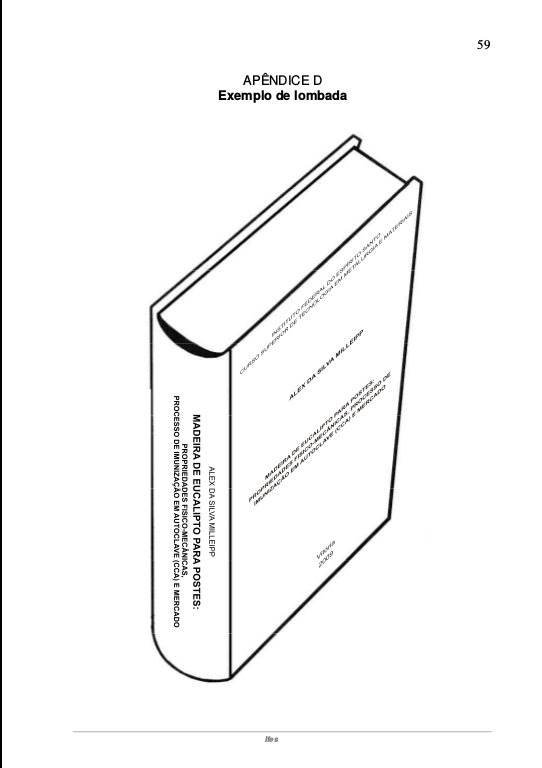
\includegraphics[scale=0.8]{pics/normas-ifes-apendice-d.png}}


\end{document}
%%% Local Variables:
%%% mode: latex
%%% TeX-master: t
%%% ispell-local-dictionary: "brasileiro"
%%% End:
